\documentclass[]{article}
\usepackage[german]{babel}
\usepackage{graphicx}
\usepackage{tabularx}
\usepackage[backend=bibtex, natbib=true]{biblatex}
\usepackage{listings}
\usepackage{tikz}

\lstset{%
	basicstyle=\ttfamily\scriptsize,        % Code font, Examples: \footnotesize, \ttfamily
	keywordstyle=\color{blue!80!black},     % Keywords font ('*' = uppercase)
	commentstyle=\color{gray},              % Comments font
	numbers=left,                           % Line nums position
	numberstyle=\tiny,                      % Line-numbers fonts
	stepnumber=1,                           % Step between two line-numbers
	numbersep=5pt,                          % How far are line-numbers from code
	backgroundcolor=\color{gray!10!white},  % Choose background color
	frame=none,                             % A frame around the code
	tabsize=2,                              % Default tab size
	captionpos=b,                           % Caption-position = bottom
	breaklines=true,                        % Automatic line breaking?
	breakatwhitespace=false,                % Automatic breaks only at whitespace?
	showspaces=false,                       % Dont make spaces visible
	showstringspaces=false                  %
	showtabs=false,                         % Dont make tabls visible
	columns=flexible,                       % Column format
	morekeywords={},                        % Specific keywords
	stringstyle=\color{green!50!black},%
}%

\bibliography{bibliography}
%opening
%Here you can enter your names and titleof your report
\title{Weekly Reports}
\author{Luftqualität in Innenräumen - Gruppe 1}

\begin{document}

\maketitle

\begin{table}[h!]
	\centering
	\begin{tabular}{|c|c|c|}
		\hline
		{\textbf{Name}}				&		{\textbf{Matrikel Nr.}} & {\textbf{Arbeitsaufwand (h)}} \\
		\hline
		Friedrich Just				&		1326699 				&	18,00	\\
		\hline
		Stipe Knez				&		1269206 				&	17,00	\\
		\hline
		Lucas Merkert				&		1326709					&	17,00	\\
		\hline
		Achim Glaesmann				&		1309221					&	19,00	\\
		\hline
		Max-Rene Konieczka			&		1211092					&	16,00	\\
		\hline
		Can Cihan Nazlier			&		1179244					&	19,00	\\
		\hline
	\end{tabular}
	\caption{Arbeitsaufwand dieser Woche}
	\label{tab:worakload}
\end{table}



\section{Überblick}


\subsection{Friedrich Just}
Der SCD41 Sensor hat die I$^2$C-Bus Adresse 0x62~\cite{datasheetscd41}Seite 7. An dem Sensor sind 4 Kabel. Das grüne Kabel geht an den SDA-port (Serial Data Line). Das gelbe Kabel geht an den SCL-port (Serial Clock). Das schwarze Kabel ist der GND-port (Ground). Das rote Kabel ist an den VDD-port (Power) angeschlossen~\cite{sht21cableconf}.\par Mit dem hexadezimal (von nun an hex.) Code 0x21b1 wird alle 5 Sekunden eine Messung durchgeführt, mit dem hex. Code 0xec05 wird die periodische Messung beendet. Wenn der Sensor den hex. Code 0xec05 sendet, bekommt er das Ergebnis der Messung zurück. Das sind die wichtigsten Kommandos für das Auslesen des Sensors die vollständige Liste siehe {Abbildung \ref{img:scd41_commandset}}.\par Für jeden Messwert werden 3 Byte eingelesen, davon sind 2 Byte Messauflösung und 1 Byte CRC (Cyclic Redundancy Check) checksum für die Fehlererkennung. Dies und die Umrechnung der Messwerte in eine lesbare Form werden in der Tabelle {Abbildung \ref{img:scd41_umrechnung}} dargestellt.\par Für ein besseres Verständnis der Programmierung des Sensors wurde dieser an einem Arduino Nano angeschlossen. Auf Github gibt es bereits einen funktionierenden Code zum Auslesen dieses Sensors und die Umrechnung der Messwerte. Damit ist verständlicher geworden, wie der Sensor über unseren Microcontroller angesteuert werden muss. Durch den Arduino kann man später die Messwerte mit denen des Microcontrollers vergleichen werden.

\begin{figure}[!h]
	\centering
	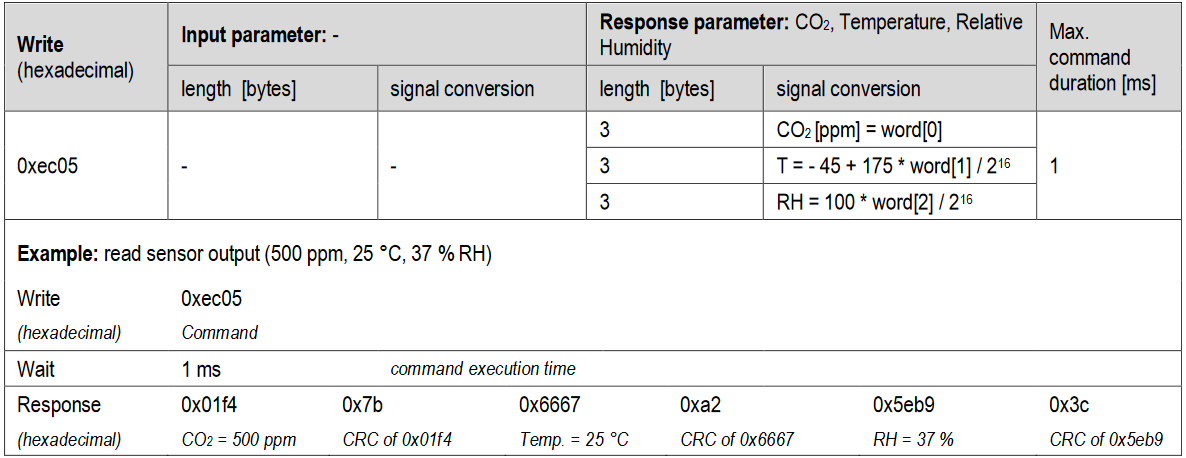
\includegraphics[scale=0.40]{images/scd41_umrechnung}
	\caption{Auswertung einer Messung ~\cite{datasheetscd41}}
	\label{img:scd41_umrechnung}
\end{figure}
\begin{figure}[!h]
	\centering
	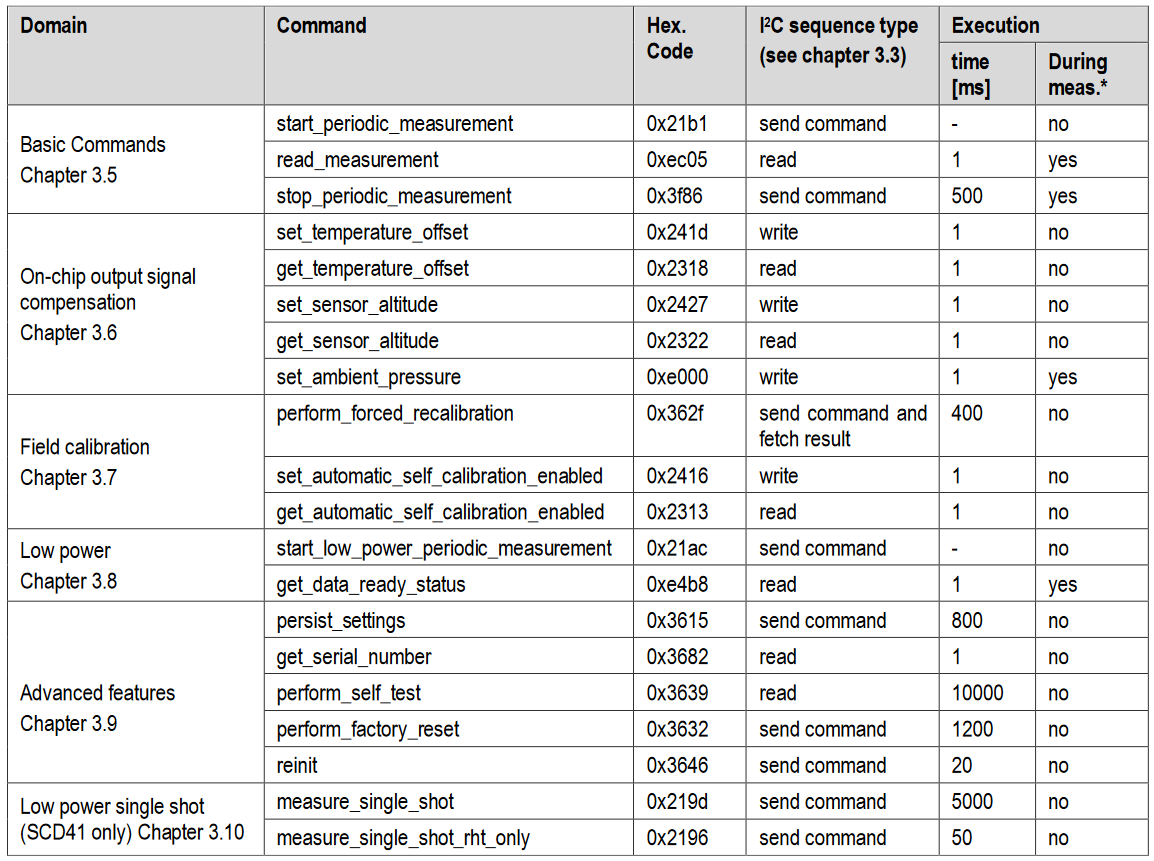
\includegraphics[scale=0.40]{images/scd41_commandset}
	\caption{Befehle zum Ansteuern des SCD41 Sensors~\cite{datasheetsht21}}
	\label{img:scd41_commandset}
\end{figure}

\subsection{Lucas Merkert}
\label{lucas}
Einarbeitung SHT21: Der SHT21 Sensor wird über den I$^2$C-Bus angesprochen {Abbildung \ref{img:sht21_commandset}} um die Temperatur und relative Luftfeuchtigkeit zu messen. Der Sensor gibt die Temperatur in einer 14 Bit Auflösung und die Relative Luftfeuchtigkeit in einer 12 Bit Auflösung zurück. Die Werte können dann mit den Formel aus {Abbildung \ref{img:sht21_tempformula}} und {Abbildung \ref{img:sht21_rhformula}} berechnet werden. Dabei ist das Problem aufgetreten wie genau man den Sensor über HAL\_WriteI2cPacket() anspricht. Mit der Lösung aus dem Forumpost sollte sich dies geklärt haben.

\begin{figure}[h]
	\centering
	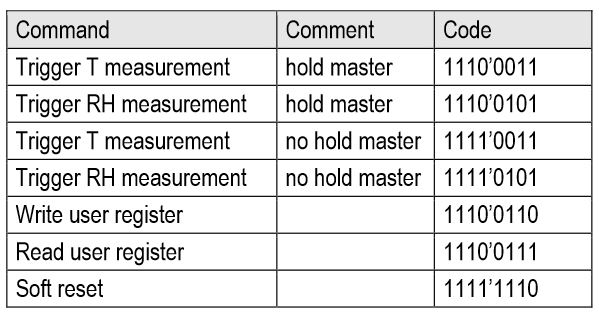
\includegraphics[scale=0.60]{images/sht21_commandset}
	\caption{Befehle zum Ansteuern des SGT21 Sensors, T für Temperatur, RH für relative Luftfeuchtigkeit~\cite{datasheetsht21}}
	\label{img:sht21_commandset}
\end{figure}
\begin{figure}[h]
	\centering
	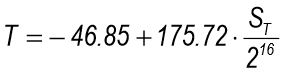
\includegraphics[scale=0.60]{images/sht21_tempformula}
	\caption{Formel zur Berechnung der Temperatur~\cite{datasheetsht21}}
	\label{img:sht21_tempformula}
\end{figure}
\begin{figure}[h]
	\centering
	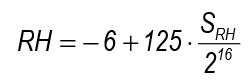
\includegraphics[scale=0.60]{images/sht21_rhformula}
	\caption{Formel zur Berechnung der relativen Luftfeuchtigkeit~\cite{datasheetsht21}}
	\label{img:sht21_rhformula}
\end{figure}

\textbf{Luftqualitäts Faktoren}~\cite{faktoren_luftquali}
\begin{itemize}
	\item Luftfeuchte
	\begin{enumerate}
		\item $>23$\% =$>$ Feuchtigkeitsverlust beim Atmen nur noch bedingt kompensierbar, Bauschäden, höhere Chance auf Elektroschocks
		\item $>40$\% =$>$ austrocknen der Haut, Schleimhaut und Augen
		\item $<60$\% =$>$ Schimmelbildung =$>$ Asthma, Allergien
		\item $<80$\% =$>$ optimale Feuchtigkeit für Milben, Parasiten, Pilzen
	\end{enumerate}
	\item VOC
	\begin{enumerate}
		\item Emissionsquellen: Bauprodukte, Möbel, Lack, Lösungsmittel verdunsten, Tabakrauch, Menschen, Tiere, Mikroorganismen höheres Risiko bei Neubau/Renovierung
		\item Schäden. Geruchsbelästigung, Atemwegs-/Augenreiz, Schädigung des Nervensystems, Allergien, Krebs, Erbgutschädigung, Fortpflanzungsschädigen
		\item RW 1: lebenslange Aussetzung führt zu keine Auswirkung (>0,3mg/m$^3$)
		\item RW 2: Schäden bei anfälligen Leuten sind zu erwarten
		\item RW gilt für alle Räume in denen keine Gefahrenstoffe verwendet werden
		\item VOC misst die gesamt Anzahl der Partikel in der Luft, einzelne Partikel könne daraus nicht abgelesen werden
	\end{enumerate}
	\item Feinstaub
	\begin{enumerate}
		\item Arten von Feinstaub: PM10, PM2.5, PM0.1 (Mikrometer)
		\item Je kleiner die Partikel desto weiter können diese in den Körper, vor allem die Lunge eindringen und diese beschädigen
		\item Emissionsquellen: Tabakrauch, Kerzenruß, Kochen, Computer, Drucker, Heizen ohne lüften
		\item Maßnahmen: saugen, wischen(nass!), lüften, nicht mehr als 22C heizen, Dunstabzugshaube in der Küche, Luftreiniger
	\end{enumerate}
\end{itemize}

\subsection{Stipe Knez}
Diese Woche spielte das Einarbeiten in das Projekt und die Vorbereitung auf das Erstellen von Mock-Daten mit Python und eine Recherche was das Express.js-Framework angeht bei mir eine Rolle.
Nach dem tieferen Einarbeiten in das Projekt (unter Anderem in die Programmiersprache) ging es an die Recherche bezüglich des Express-Frameworks, da dieses in unserem Projekt eine Rolle spielen soll und dementsprechend Wissen über die Funktionsweise und Nutzungsweise benötigt wird. Das Express.js-Framework ist dabei ein serverseitiges Web-Framework für die JavaScript-basierte Plattform Node.js. Durch dieses Framework werden in Node.js Werkzeuge zur Verfügung gestellt, durch die sich Webanwendungen leichter entwickeln lassen~\cite{Express.js}. Node.js ist dabei eine  plattformübergreifende JavaScript-Laufzeitumgebung, die in der Lage ist Javascript-Programme außerhalb des Webbrowsers ausführen zu lassen~\cite{Node.js}.
Wie zuvor erwähnt, war die Vorbereitung auf das Erstellen von Mock-Daten mit Python auch ein Bestandteil der Arbeit in der letzten Woche. Wir möchten mit Hilfe von Python Mock-Daten zum Testen erstellen, die weiterverarbeitet werden sollen. Die damit einhergehende Recherche hat Aufschluss über die Herangehensweise beim Erstellen von Mock-Daten gegeben. Für die kommende Woche ist geplant, dieses Wissen umzusetzen und in Zusammenarbeit mit dem für die ZigBee-Daten verantwortlichen Team, das passende Format für die Daten zu wählen und diese schließlich zu erstellen~\cite{mockdata}.

\subsection{Achim Glaesmann}
Es wurde daran gearbeitet die Sensoren mit dem Mikrokontroller auszulesen. Das Auslesen bereitet jedoch unvorhergesehene Probleme. Die Datenblätter wurden ausführlich studiert um eine
Kommunikation über I2C zu ermöglichen. ~\cite{datasheetcss811}~\cite{datasheetscd41}~\cite{datasheetsht21} Es wurden die Befehle recherchiert und die für die Berechnungen der Werte nötigen Umrechnungsformeln der Sensordaten. {[\ref{img:sht21_commandset}]}  {[\ref{img:sht21_tempformula}]} {[\ref{img:sht21_rhformula}]} Das I2C Protokoll wurde ausführlich studiert. Die in den Datenblättern vermerkten Adressen der Sensoren führen jedoch nicht zu dem Aufbau einer 
Verbindung. Zur Fehleranalyse wurde ein Skript für den Arduino entwickelt um die Verbindung mit über I2C zu kontrollieren. Über den Arduino war es möglich eine Verbindung herzustellen.
Es wurde ein Skript herangezogen, welches es ermöglicht die 7 bit I2C Adressen zu überprüfen um Abweichungen vom Datenblatt zu erkennen. Beim SHT21 Sensor wurde eine Abweichung festgestellt.
Eine Verwendung der so herausgefundenen I2C Adresse führte allerdings ebenfalls zu einem OpenFail. Es wurde ein Übertragungsstandard für die von den Sensoren ermittelten Daten über
die UART-Schnittstelle entwickelt. Es ist geplant die Daten durch ein Semikolon getrennt in einer vorher festgelegten Reihenfolge zu übertragen. Dabei erhält jeder Mikrokontroller eine
ID, die gemeinsam mit den ermittelten Daten übertragen wird. Der Aufbau wäre vorraussichtlich wie folgt: (ID; DATASENSOR1; DATASENSOR2; DATASENSOR3) Bei Multisensoren erfolgt die Weitergabe
der Daten in Reihenfolge der Sensoren durch ein Semikolon getrennt. DATASENSOR1 wäre im Falle des SHT21 dann wie folgt aufgeteilt: TEMPERATURCELSIUS; LUFTFEUCHTIGKEITRH;. Es wurde weiter
die Literatur studiert, um einen Überblick über Sinnvolle Gefahrenabschätzung auf Basis der vorliegenden Daten zu erhalten. ~\cite{faktoren_luftquali} [\ref{lucas}] Endgültige Grenzwerte werden weiter recherchiert, 
eine Entscheidung wird später getroffen, da das Software Team sich bisher hauptsächlich auf das Zeichentool konzentriert, empfiehlt es sich weitere Informationen einzuholen, bis
die Entwicklung an dem Punkt ist, an dem die Gefahreneinschätzung etabliert werden muss.

\subsection{Max-Rene Konieczka}
Aufbauend zur letzten Woche, hat man sich mit der korrekten Einrichtung ein Einarbeitung des Projektes beschäftigt, welches von Can Cihan Nazlier letzte Woche konfiguriert wurde. Darüber hinaus wurde influxDB installiert, was sich gut dafür eignet Zeitreihen-Daten zu verwalten. Da die Applikation eine Reactive Web App sein wird, wurden Recherchen zum Thema Websockets und SocketIO gemacht. SocketIO ist eine JavaScript-Bibliothek, welche für Echtzeit-Webanwendungen verwendet wird. Diese ermöglicht bidirektionale Echtzeit-Kommunikation zwischen dem Browser und einem Server. Dadurch werden Benutzereingaben schneller behandelt und die App läuft flüssiger.~\cite{socketIO1, socketIO2} Websocket wiederum ist ein Netzwerkprotokoll, was auf TCP basiert und die Kommunikation überhaupt möglich macht. SocketIO macht sich das WebSocket-Protokoll zunutze.~\cite{webSocket1, webSocket2} Für die kommende Woche wird versucht, die im Zeichentool eingezeichneten Räume persistent zu speichern, sodass das diese nach der Schließung und erneuten Ausführung des Tools wieder verfügbar sind. 

\subsection{Can Cihan Nazlier}
Diese Woche wurde der Prototyp des Zeichentools fertiggestellt, nachdem mit Herrn Krauße über Einzelheiten am Dienstag gesprochen wurde. Man kann nun Räume erstellen und diese abspeichern(noch nicht persistent). Nach der Abspeicherung, verändert sich die Farbe der Räume auf dem Zeichenboard von Rot auf Grün. Im Verlauf nächster Woche wird daran gearbeitet die Räume persistent abzuspeichern, sei es in eine .json Datei oder in einer Datenbank. Nächste Woche wird dazu noch am Menü gearbeitet, welches gespeicherte Räume anzeigen und der Nutzer diese bearbeiten können soll. 
Eine geeignete Ticketumgebung um die Übersicht für die Entwickler zu erhalten wurde konfiguriert. Benutzt wird die Applikation 'Trello'. Zwei Boards wurden eingerichtet, jeweils eins für den Backend- und Frontend-Teil.

\printbibliography
%----------------------------------------------------------------------------
% Bibliography
%----------------------------------------------------------------------------	
\end{document}
